\documentclass[conference]{IEEEtran}
\IEEEoverridecommandlockouts
\usepackage{url}
\usepackage{cite}
\usepackage{amsmath,amssymb,amsfonts}
\usepackage{booktabs}
\usepackage{graphicx}
\usepackage{textcomp}
\usepackage{xcolor}
% numbers.tex and tables.tex are generated by make_report_assets.py from results/ and report/evidence/
% generated by make_report_assets.py, do not edit
\newcommand{\ConfFN}{11{,}032}
\newcommand{\ConfFP}{5{,}616}
\newcommand{\ConfTN}{30{,}602}
\newcommand{\ConfTP}{106{,}497}
\newcommand{\ConfigEpochs}{10}
\newcommand{\ConfigSeed}{42}
\newcommand{\DupAccBound}{0.9990}
\newcommand{\DupConflictRows}{9{,}473}
\newcommand{\DupConflictVecs}{440}
\newcommand{\DupDistinct}{1{,}257{,}385}
\newcommand{\DupRepeats}{277{,}700}
\newcommand{\DupRows}{1{,}535{,}085}
\newcommand{\DupSeenBenignPct}{0.6}
\newcommand{\DupSeenMalPct}{27.9}
\newcommand{\DupSeenMax}{21.7}
\newcommand{\DupSeenMin}{21.5}
\newcommand{\DupSeenOrig}{65{,}867}
\newcommand{\DupSeenOrigPct}{21.45}
\newcommand{\FamBenignErr}{33.7}
\newcommand{\FamBenignRate}{0.845}
\newcommand{\FamBruteForceErr}{2.3}
\newcommand{\FamBruteForceRate}{0.710}
\newcommand{\FamDDoSErr}{0.0}
\newcommand{\FamDDoSRate}{1.000}
\newcommand{\FamMiraiErr}{0.0}
\newcommand{\FamMiraiRate}{1.000}
\newcommand{\FamReconErr}{44.3}
\newcommand{\FamReconRate}{0.596}
\newcommand{\FamSpoofingErr}{17.1}
\newcommand{\FamSpoofingRate}{0.905}
\newcommand{\FamWebbasedErr}{2.5}
\newcommand{\FamWebbasedRate}{0.524}
\newcommand{\HoldBruteForceOut}{0.614}
\newcommand{\HoldBruteForceSeen}{0.710}
\newcommand{\HoldDDoSOut}{1.000}
\newcommand{\HoldDDoSSeen}{1.000}
\newcommand{\HoldMiraiOut}{1.000}
\newcommand{\HoldMiraiSeen}{1.000}
\newcommand{\HoldReconOut}{0.392}
\newcommand{\HoldReconSeen}{0.596}
\newcommand{\HoldSpoofingOut}{0.171}
\newcommand{\HoldSpoofingSeen}{0.905}
\newcommand{\HoldWebbasedOut}{0.495}
\newcommand{\HoldWebbasedSeen}{0.524}
\newcommand{\MainAP}{0.9875}
\newcommand{\MainAcc}{0.8917}
\newcommand{\MainAuc}{0.9560}
\newcommand{\MainBalAcc}{0.8755}
\newcommand{\MainBenignFOne}{0.7862}
\newcommand{\MainBenignPrec}{0.7350}
\newcommand{\MainBenignRec}{0.8449}
\newcommand{\MainFOne}{0.9275}
\newcommand{\MainMacroFOne}{0.8568}
\newcommand{\MainMacroPrec}{0.8425}
\newcommand{\MainMacroRec}{0.8755}
\newcommand{\MainMajority}{0.7644}
\newcommand{\MainPrec}{0.9499}
\newcommand{\MainRec}{0.9061}
\newcommand{\NTest}{153{,}747}
\newcommand{\NTrain}{1{,}227{,}810}
\newcommand{\NVal}{153{,}528}
\newcommand{\OrigAcc}{0.8879}
\newcommand{\OrigAuc}{0.9555}
\newcommand{\OrigFOne}{0.9230}
\newcommand{\OrigPrec}{0.9709}
\newcommand{\OrigRec}{0.8796}
\newcommand{\OrigSeenAcc}{0.9950}
\newcommand{\OrigSeenFOne}{0.9975}
\newcommand{\OrigSeenRec}{0.9999}
\newcommand{\OrigSeenShare}{21.6}
\newcommand{\OrigUnseenAcc}{0.8622}
\newcommand{\OrigUnseenFOne}{0.8987}
\newcommand{\OrigUnseenRec}{0.8722}
\newcommand{\OrigUnseenShare}{78.4}
\newcommand{\OurMargin}{12.7}
\newcommand{\PaperAcc}{0.9944}
\newcommand{\PaperFOne}{0.9403}
\newcommand{\PaperImpliedBenignRec}{0.8691}
\newcommand{\PaperImpliedMalRec}{0.9974}
\newcommand{\PaperMajority}{0.9765}
\newcommand{\PaperMalPosAccBound}{0.9348}
\newcommand{\PaperMargin}{1.8}
\newcommand{\PaperPrec}{0.9476}
\newcommand{\PaperRec}{0.9333}
\newcommand{\RunDevice}{NVIDIA GeForce RTX 2070 SUPER}
\newcommand{\RunSeconds}{658}
\newcommand{\SeedsBothGroupedAccMean}{0.8908}
\newcommand{\SeedsBothGroupedAccSd}{0.0018}
\newcommand{\SeedsBothGroupedFOneMean}{0.9269}
\newcommand{\SeedsBothGroupedFOneSd}{0.0011}
\newcommand{\SeedsBothGroupedN}{5}
\newcommand{\SeedsBothGroupedRecMean}{0.9059}
\newcommand{\SeedsBothGroupedRecSd}{0.0087}
\newcommand{\SeedsBothRandomAccMean}{0.8908}
\newcommand{\SeedsBothRandomAccSd}{0.0018}
\newcommand{\SeedsBothRandomFOneMean}{0.9270}
\newcommand{\SeedsBothRandomFOneSd}{0.0011}
\newcommand{\SeedsBothRandomN}{5}
\newcommand{\SeedsBothRandomRecMean}{0.9079}
\newcommand{\SeedsBothRandomRecSd}{0.0087}
\newcommand{\SweepBestArch}{128/64/32}
\newcommand{\SweepBestF}{0.9288}
\newcommand{\SweepBestLr}{0.001}
\newcommand{\SweepBestWeights}{unweighted}
\newcommand{\SweepChosenIsBest}{yes}
\newcommand{\SweepEpochs}{10}
\newcommand{\SweepLrOneMax}{0.9288}
\newcommand{\SweepLrOneMin}{0.9267}
\newcommand{\SweepLrThreeMax}{0.9246}
\newcommand{\SweepRuns}{12}
\newcommand{\SweepSpread}{0.0021}
\newcommand{\SweepWeightedF}{0.9121}
\newcommand{\SweepWeightedPrec}{0.9889}
\newcommand{\SweepWeightedRec}{0.8464}
\newcommand{\TestMalPct}{76.4}
\newcommand{\TestSeenInTrain}{0}
\newcommand{\ValAcc}{0.8936}
\newcommand{\ValAuc}{0.9569}
\newcommand{\ValFOne}{0.9288}
\newcommand{\ValPrec}{0.9507}
\newcommand{\ValRec}{0.9079}

% generated by make_report_assets.py, do not edit
\newcommand{\tabHoldout}{\begin{table}[t]\centering\caption{Detection rate on each attack family's test rows when the family is in training versus withheld from training, with benign specificity for both models (same seed and split).}\label{tab:holdout}\footnotesize\setlength{\tabcolsep}{3pt}
\begin{tabular}{@{}lrcccc@{}}\toprule
Family & Rows & Seen & Held out & Spec. seen & Spec. held out \\ \midrule
Brute Force & 1{,}325 & 0.710 & 0.614 & 0.845 & 0.843 \\
DDoS & 60{,}063 & 1.000 & 1.000 & 0.845 & 0.833 \\
Mirai & 6{,}951 & 1.000 & 1.000 & 0.845 & 0.821 \\
Recon & 18{,}266 & 0.596 & 0.392 & 0.845 & 0.940 \\
Spoofing & 30{,}040 & 0.905 & 0.171 & 0.845 & 0.967 \\
Web-based & 884 & 0.524 & 0.495 & 0.845 & 0.852 \\
\bottomrule\end{tabular}\end{table}}
\newcommand{\tabMain}{\begin{table*}[t]\centering\caption{Test results. Ours: grouped split, malicious as positive class, threshold 0.5. ``Original'': same code on the original random 80/20 split (a fresh run of the original protocol / the submitted numbers). Macro: unweighted mean over the two classes (\textsuperscript{b} balanced accuracy). Paper: two-class DNN, Table 6 of Neto et al.; \textsuperscript{c} computed from its Table 3 benign share (1{,}098{,}195 of 46{,}686{,}579 rows).}\label{tab:main}\footnotesize\setlength{\tabcolsep}{3pt}
\begin{tabular}{@{}lccccc@{}}\toprule
Metric & Ours & Orig.\ (rerun) & Orig.\ (submitted) & Ours, macro & Paper DNN \\ \midrule
Accuracy & 0.8917 & 0.8902 & 0.8879 & 0.8755\textsuperscript{b} & 0.9944 \\
Precision & 0.9499 & 0.9580 & 0.9709 & 0.8425 & 0.9476 \\
Recall & 0.9061 & 0.8955 & 0.8796 & 0.8755 & 0.9333 \\
F1 & 0.9275 & 0.9257 & 0.9230 & 0.8568 & 0.9403 \\
ROC-AUC & 0.9560 & 0.9555 & 0.9555 & -- & -- \\
Always-malicious accuracy & 0.7644 & -- & -- & -- & 0.9765\textsuperscript{c} \\
\bottomrule\end{tabular}\end{table*}}
\newcommand{\tabSeeds}{\begin{table}[t]\centering\caption{Test metrics over seeds (mean $\pm$ sd). The seed changes the split and the initialisation.}\label{tab:seeds}\footnotesize\setlength{\tabcolsep}{3pt}
\begin{tabular}{@{}lrccccc@{}}\toprule
Protocol & Runs & Acc & Prec & Rec & F1 & AUC \\ \midrule
grouped split & 5 & 0.8908$\pm$0.0018 & 0.9490$\pm$0.0092 & 0.9059$\pm$0.0087 & 0.9269$\pm$0.0011 & 0.9555$\pm$0.0009 \\
original random split & 5 & 0.8908$\pm$0.0018 & 0.9471$\pm$0.0092 & 0.9079$\pm$0.0087 & 0.9270$\pm$0.0011 & 0.9554$\pm$0.0008 \\
\bottomrule\end{tabular}\end{table}}
\newcommand{\tabSeen}{\begin{table}[t]\centering\caption{Original random 80/20 split, test rows grouped by whether the row's exact feature vector also occurs in training (mean over 5 seeds).}\label{tab:seen}\footnotesize\setlength{\tabcolsep}{3pt}
\begin{tabular}{@{}lrcccc@{}}\toprule
Test rows & Share & Acc & Prec & Rec & F1 \\ \midrule
twin in training & 21.6\% & 0.9950 & 0.9951 & 0.9999 & 0.9975 \\
no twin in training & 78.4\% & 0.8622 & 0.9272 & 0.8722 & 0.8987 \\
all test rows & 100\% & 0.8908 & 0.9471 & 0.9079 & 0.9270 \\
\bottomrule\end{tabular}\end{table}}
\newcommand{\tabSource}{\begin{table*}[t]\centering\caption{Grouped test partition by source file: fraction classified correctly (detection rate for attacks, specificity for benign), share of all test errors, and share of that file's rows in the dataset that repeat an earlier feature vector.}\label{tab:source}\footnotesize\setlength{\tabcolsep}{3pt}
\begin{tabular}{@{}llrccr@{}}\toprule
File & Family & Rows & Correct & Errors & Repeats \\ \midrule
BenignTraffic & Benign & 36{,}218 & 0.845 (specificity) & 33.7\% & 0.4\% \\
DictionaryBruteForce & Brute Force & 1{,}325 & 0.710 (detection) & 2.3\% & 0.0\% \\
DDoS-ICMP\_Flood & DDoS & 15{,}113 & 1.000 (detection) & 0.0\% & 44.1\% \\
DDoS-SYN\_Flood & DDoS & 15{,}112 & 1.000 (detection) & 0.0\% & 28.9\% \\
DDoS-TCP\_Flood & DDoS & 15{,}014 & 1.000 (detection) & 0.0\% & 50.5\% \\
DDoS-UDP\_Flood & DDoS & 14{,}824 & 1.000 (detection) & 0.0\% & 46.7\% \\
Mirai-greeth\_flood & Mirai & 3{,}317 & 1.000 (detection) & 0.0\% & 0.5\% \\
Mirai-udpplain & Mirai & 3{,}634 & 1.000 (detection) & 0.0\% & 0.3\% \\
Recon-OSScan & Recon & 9{,}935 & 0.552 (detection) & 26.7\% & 1.8\% \\
Recon-PortScan & Recon & 8{,}331 & 0.648 (detection) & 17.6\% & 2.5\% \\
DNS\_Spoofing & Spoofing & 14{,}846 & 0.908 (detection) & 8.2\% & 2.5\% \\
MITM-ArpSpoofing & Spoofing & 15{,}194 & 0.903 (detection) & 8.9\% & 7.4\% \\
SqlInjection & Web-based & 498 & 0.482 (detection) & 1.5\% & 0.0\% \\
XSS & Web-based & 386 & 0.578 (detection) & 1.0\% & 0.0\% \\
\bottomrule\end{tabular}\end{table*}}
\newcommand{\tabSweep}{\begin{table}[t]\centering\caption{Validation sweep (10 epochs each), sorted by validation F1. $\ast$ marks the configuration in config.yaml. The test partition was not scored.}\label{tab:sweep}\footnotesize\setlength{\tabcolsep}{3pt}
\begin{tabular}{@{}lcccccc@{}}\toprule
Hidden & LR & Loss & Prec & Rec & F1 & AUC \\ \midrule
128/64/32$\ast$ & 0.001 & plain & 0.9507 & 0.9079 & 0.9288 & 0.9569 \\
128/64 & 0.001 & plain & 0.9403 & 0.9167 & 0.9283 & 0.9560 \\
256/128/64 & 0.001 & plain & 0.9325 & 0.9237 & 0.9281 & 0.9561 \\
64/64 & 0.001 & plain & 0.9454 & 0.9097 & 0.9272 & 0.9556 \\
256/128 & 0.001 & plain & 0.9592 & 0.8964 & 0.9267 & 0.9562 \\
128/64 & 0.003 & plain & 0.9404 & 0.9094 & 0.9246 & 0.9525 \\
128/64/32 & 0.003 & plain & 0.9395 & 0.9101 & 0.9246 & 0.9526 \\
64/64 & 0.003 & plain & 0.9419 & 0.9073 & 0.9243 & 0.9522 \\
256/128 & 0.003 & plain & 0.9575 & 0.8884 & 0.9216 & 0.9519 \\
256/128/64 & 0.003 & plain & 0.9075 & 0.9360 & 0.9215 & 0.9514 \\
128/64 & 0.001 & weighted & 0.9889 & 0.8464 & 0.9121 & 0.9561 \\
128/64 & 0.003 & weighted & 0.9924 & 0.8196 & 0.8978 & 0.9510 \\
\bottomrule\end{tabular}\end{table}}

\begin{document}

\title{Binary Intrusion Detection on a CICIoT2023 Subset With a Deep Neural Network}

\author{\IEEEauthorblockN{Willis Martin}
\IEEEauthorblockA{\textit{Department of Cybersecurity} \\
\textit{Rochester Institute of Technology}\\
Rochester, NY, USA \\
wrm3207@rit.edu}
}

\maketitle

\begin{abstract}
This project trains a small neural network to label CICIoT2023 network flows as benign or malicious. The training table has \DupRows{} flows built from 14 of the dataset's per-attack files: benign traffic and 13 attack types from six of the dataset's seven categories (no DoS files). Feature vectors repeat heavily in this table, mostly in DDoS traffic, so a plain random split leaves an exact copy of \DupSeenOrigPct\% of the test rows in the training set. I split by feature vector into training, validation and test partitions, chose hyperparameters on the validation partition only, and scored the test partition once. On \NTest{} test rows the model reaches accuracy \MainAcc, precision \MainPrec, recall \MainRec, F1 \MainFOne{} and ROC-AUC \MainAuc. Grouping did not move the aggregate scores (F1 \SeedsBothGroupedFOneMean{} grouped against \SeedsBothRandomFOneMean{} on the original split, five seeds each). The aggregate hides large gaps, though: DDoS and Mirai flows are detected perfectly, Recon scans at \FamReconRate, and holding the spoofing family out of training drops its detection from \HoldSpoofingSeen{} to \HoldSpoofingOut. The paper's two-class DNN reports F1 0.9403, but its data are 97.6\% malicious against \TestMalPct\% here, so accuracy cannot be compared across the two setups.
\end{abstract}

\begin{IEEEkeywords}
intrusion detection, deep neural network, IoT security, CICIoT2023, evaluation validity
\end{IEEEkeywords}

\section{Introduction}
IoT devices are a growing attack surface, and flow-level classifiers are a common first line of detection. This project trains and evaluates a deep neural network on CICIoT2023 \cite{s23135941} to separate benign flows from malicious ones, and compares the result with the benchmark in the dataset paper.

The main design question was how to evaluate fairly. The dataset paper uses a random 80/20 split. On the table I assembled, that split puts an exact feature-vector copy of about a fifth of the test rows into training, and an earlier version of this project also compared several configurations on the test split. Both are known evaluation pitfalls in security machine learning \cite{arp2022dos}. This version separates the partitions by feature vector, selects on validation data, and reports how much the original protocol changes the numbers.

\section{Background and Related Work}
CICIoT2023 \cite{s23135941} contains 33 attacks in seven categories (DDoS, DoS, Recon, Web-based, brute force, spoofing, Mirai), executed by IoT devices against other IoT devices in a topology of 105 devices. Table~4 of the paper lists 47 features, of which only the timestamp is removed before modelling. For machine learning the paper blends all files, splits 80\% training and 20\% test at random, standardizes with StandardScaler, and evaluates five models for 2, 8 and 34 classes. Its two-class DNN scores accuracy 0.9944, precision 0.9476, recall 0.9333 and F1 0.9403 (Table~6). In the passages I checked the paper does not state how precision, recall and F1 are averaged for the two-class task and does not describe the DNN's size.

Salman and Yong \cite{salman2025overview} survey the dataset and note its use as a baseline for binary and multi-class studies, with size as both a strength and an obstacle for reproduction on limited hardware. Evaluation problems in public intrusion datasets are well documented. Engelen et al. \cite{engelen2021troubleshooting} found flow-construction and labelling errors in CICIDS2017, another CIC dataset, that materially change reported detection performance. Arp et al. \cite{arp2022dos} list sampling bias and data snooping (using test data for any part of model building) among the common pitfalls in learning-based security research. Both are relevant to the setup below.

\section{Data and Methods}
\subsection{Source files and assembly}
I used the benign file and 13 attack files from the CIC server: DDoS ICMP, SYN, TCP and UDP floods, dictionary brute force, DNS spoofing, ARP spoofing (MITM), Mirai GRE-ETH flood, Mirai UDPPlain, OS scan, port scan, SQL injection and XSS. That is 13 of the 33 attacks in Table~3 of the paper and six of its seven categories. \emph{No DoS file was downloaded}, so the DoS category, and the 20 other attacks, are absent. Several files also hold only part of an attack's rows (the ICMP flood file has 268{,}010 rows against 7{,}200{,}504 in the paper's Table~3, and the benign file 362{,}361 against 1{,}098{,}195). The dictionary brute force, OS scan, port scan, SQL injection and XSS files match the paper's row counts.

Each attack file is capped at 150{,}000 randomly chosen rows (seed 42). The cap is per file, not per category, and only six files exceed it (four DDoS floods, DNS spoofing and ARP spoofing). Rows with infinite or missing values (52) are dropped and the result is shuffled. The table has \DupRows{} rows, 362{,}342 benign and 1{,}172{,}743 malicious (3.2:1). It has 39 numeric features. Compared with the 46 non-timestamp features of Table~4 in the paper, the files lack flow\_duration, Srate, Drate, urg\_count, Magnitue, Radius, Covariance and Weight and add an IGMP indicator. I do not know why the distributed files differ, and I did not test what the missing features would change.

\texttt{data/build\_dataset.py} rebuilds this table from the raw files byte for byte and refuses to run if any declared file is missing. The pinned SHA-256 of the result is checked by the downloader and by the training code, so a different or truncated \texttt{dataset.csv} is rejected rather than silently used.

\subsection{Repeated feature vectors}
\DupRepeats{} of the \DupRows{} rows repeat an earlier row's exact feature vector, leaving \DupDistinct{} distinct vectors. The repeats sit almost entirely in malicious traffic and mostly in the DDoS floods (Table~\ref{tab:source}, last column). A further \DupConflictVecs{} vectors (\DupConflictRows{} rows) occur with both labels, which caps the accuracy of any classifier at \DupAccBound. That cap is far above the scores here, so label conflicts do not explain the errors.

\subsection{Partitions}
Rows with an identical feature vector form a group, and whole groups go to one partition: 80\% training, 10\% validation and 10\% test (\NTrain, \NVal{} and \NTest{} rows), stratified on each group's majority label, seed \ConfigSeed. By construction \TestSeenInTrain{} test rows have a vector that occurs in training. The StandardScaler is fitted on the training rows only. As a comparison I keep the original protocol, a stratified random 80/20 row split with no validation partition. Grouping handles exact repeats only. Near-duplicates are not detected.

\subsection{Model and training}
The model is a PyTorch MLP with two hidden layers of 128 and 64 ReLU units, dropout 0.1 and a two-way output. It is trained with cross-entropy (unweighted), Adam (learning rate $10^{-3}$, weight decay $10^{-4}$), batch size 64 and \ConfigEpochs{} epochs. Predictions use a 0.5 threshold on the malicious-class probability. The reported run took \RunSeconds{} s on \RunDevice.

\subsection{Model selection}
Architecture, learning rate and loss weighting were chosen with a sweep scored on the validation partition only (\texttt{tools/sweep.py}). The grid was fixed in advance: five architectures at two learning rates, plus class-weighted loss for the 128/64 model, and the selection criterion was validation F1. Dropout, weight decay and batch size were not varied. The test partition is scored only by the final run and by the variability runs described below, none of which feed back into any choice.

\subsection{Metrics}
Precision, recall and F1 treat malicious as the positive class. Because the paper does not state its averaging, Table~\ref{tab:main} also gives the unweighted mean of the two classes (macro average) for the same predictions. ROC-AUC uses the predicted probability.

\section{Results}
\tabMain

On the test partition (\TestMalPct\% malicious) the model labels \ConfFP{} benign flows as malicious and misses \ConfFN{} attacks, a benign specificity of \MainBenignRec{} and an attack recall of \MainRec{} (Fig.~\ref{fig:cm}).

\begin{figure}[htbp]
\centering
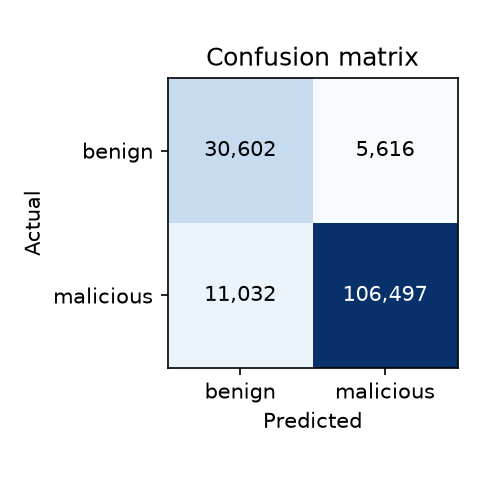
\includegraphics[width=0.48\columnwidth]{confusion_matrix.png}\hfill
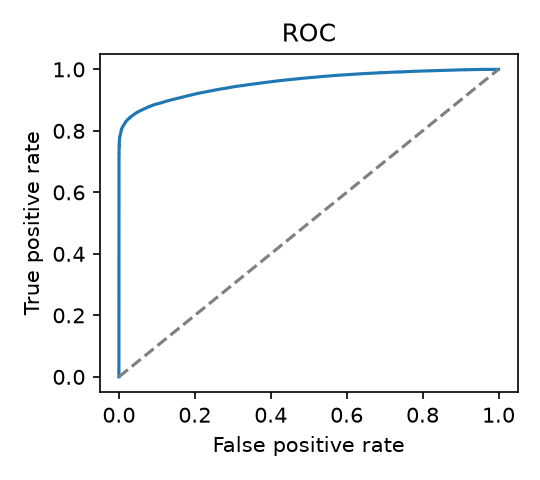
\includegraphics[width=0.48\columnwidth]{roc_curve.png}
\caption{Confusion matrix and ROC curve on the grouped test partition.}
\label{fig:cm}
\end{figure}

\subsection{Effect of the split protocol}
Splitting by feature vector did not change the aggregate result. Over five seeds the grouped protocol gives F1 \SeedsBothGroupedFOneMean{} ($\pm$\SeedsBothGroupedFOneSd) and the original random protocol \SeedsBothRandomFOneMean{} ($\pm$\SeedsBothRandomFOneSd), and accuracy is the same to four digits (Table~\ref{tab:seeds}). The original submission's headline was therefore not inflated by the repeated vectors in any way these runs can detect. What the grader's concern changes is how the number should be read. In the random split about \OrigSeenShare\% of test rows have a twin in training, and those rows are almost all malicious flood traffic that is classified nearly perfectly (F1 \OrigSeenFOne{}, Table~\ref{tab:seen}). The remaining rows score F1 \OrigUnseenFOne{} and accuracy \OrigUnseenAcc{}. The grouped test partition contains no such rows, yet its overall score is equal to the random split's overall score. That is only possible because the grouped partition is still full of easy rows: DDoS floods are about 39\% of its test rows and have no errors (Table~\ref{tab:source}). I read this as the repeated vectors mattering little for the model, because DDoS is also detected perfectly when it is withheld entirely (Table~\ref{tab:holdout}), and the row-weighted aggregate being dominated by easy traffic under both protocols. The subset comparison is also confounded by class mix (the no-twin subset is about 70\% malicious against 76\% overall), so I do not treat the seen/unseen gap as a pure leakage effect.
\tabSeen
\tabSeeds

\subsection{Where the errors come from}
Errors are concentrated. DDoS and Mirai files have no errors on the test partition. Recon scans account for \FamReconErr\% of all errors (OS scan detected at 0.552, port scan at 0.648), benign flows flagged as attacks for \FamBenignErr\% (specificity \FamBenignRate{}), and spoofing for \FamSpoofingErr\%. Brute force and the two web attacks have the lowest detection rates (\FamBruteForceRate{}, and 0.482 and 0.578 for SQL injection and XSS) but are few rows, so they contribute \FamBruteForceErr\% and \FamWebbasedErr\% of the errors; with 884 web-attack test rows those rates are also noisy. The repeated-vector share in Table~\ref{tab:source} shows where the duplicates sit: the four DDoS floods, which are also the files the model never gets wrong. The weak spots are Recon and the benign class, so a quoted overall F1 of about 0.93 mostly describes how well the model handles floods.
\tabSource

\subsection{Attack families absent from training}
For each family I retrained the same configuration with that family removed from training and scored the original test rows of the family (single seed \ConfigSeed{}, so no variance estimate). DDoS and Mirai are still detected at 1.000 when withheld, presumably because the other family's flood traffic looks similar to them, though I did not test that. The other families are not so well covered. Spoofing falls from \HoldSpoofingSeen{} to \HoldSpoofingOut, Recon from \HoldReconSeen{} to \HoldReconOut, and brute force from \HoldBruteForceSeen{} to \HoldBruteForceOut. The web attacks barely change (\HoldWebbasedSeen{} to \HoldWebbasedOut), but they were already near chance, so that is not evidence of generalization. Benign specificity rises when Recon or Spoofing is withheld (0.940 and 0.967 against 0.845), which fits the idea that these families overlap benign traffic in feature space and pull the boundary toward flagging benign flows, though this is a hypothesis I did not test directly. The practical reading is that the model recognizes the attack types it was trained on and has little ability to detect a new family, except for flood traffic.
\tabHoldout

\subsection{Hyperparameter sweep}
All \SweepRuns{} sweep runs trained for \SweepEpochs{} epochs and were scored on the validation partition only. The five architectures at learning rate 0.001 span validation F1 \SweepLrOneMin{} to \SweepLrOneMax{}, a spread of \SweepSpread{}, which is about twice the seed-to-seed standard deviation of test F1 (\SeedsBothGroupedFOneSd{}). I therefore do not claim that depth matters. The \SweepBestArch{} network is the validation-F1 winner and is the one in \texttt{config.yaml}, chosen by the criterion fixed before the sweep. Learning rate 0.003 was worse for every architecture (best \SweepLrThreeMax{}). Class-weighted loss lowers F1 to \SweepWeightedF{} because it trades recall (\SweepWeightedRec{}) for precision (\SweepWeightedPrec{}); whether that trade is better depends on the cost of missed attacks against false alarms, which this project does not model. Validation F1 and loss flatten over the last few epochs, so \ConfigEpochs{} epochs is enough for this setup.
\tabSweep

\subsection{Comparison with the paper}
Accuracy cannot be compared directly. The paper's Table~3 gives a benign share of 2.35\%, so always predicting malicious is already \PaperMajority{} accurate and its DNN's \PaperAcc{} is \PaperMargin{} points above that. Here always-malicious scores \MainMajority{} and the model's \MainAcc{} is \OurMargin{} points above it. The paper's two-class results are accuracy \PaperAcc{}, precision \PaperPrec{}, recall \PaperRec{} and F1 \PaperFOne{}, and it does not say how they are averaged. The numbers themselves give a hint. If precision and recall were for the malicious class, recall \PaperRec{} would cap accuracy at \PaperMalPosAccBound{} given a 97.6\% malicious test set, which contradicts \PaperAcc{}. Weighted averaging would make recall equal to accuracy. Macro averaging is consistent: with accuracy \PaperAcc{} it implies a benign recall near \PaperImpliedBenignRec{} and a malicious recall near \PaperImpliedMalRec{}. This is my inference from the published values, not something the paper states. On that macro reading, the comparison with this model (Table~\ref{tab:main}) is precision \MainMacroPrec{} against \PaperPrec{}, recall \MainMacroRec{} against \PaperRec{} and F1 \MainMacroFOne{} against \PaperFOne{}, so this model is below the paper's by roughly 0.06 to 0.1 depending on the metric. The implied benign recall of the paper (about \PaperImpliedBenignRec{}) is close to the \MainBenignRec{} here, so the gap comes mostly from attack detection: about \PaperImpliedMalRec{} implied against \MainRec{} here. Possible reasons, none of which I tested, are the different class mix (the paper's malicious rows are dominated by DoS and DDoS floods that are easy, while here Recon and spoofing carry the errors), a larger network or longer training on the paper's side (I did not find the paper's DNN size in the sections I checked), and the eight features missing from my files. The ROC-AUC of \MainAuc{} has no paper counterpart in the values I compared.


\subsection{Limitations}
\emph{Data coverage.} The table has 13 of 33 attack types, no DoS category, partial files for several attacks and 39 of 46 features, so the results describe this subset and are not a reproduction of the paper's benchmark. \emph{Duplicates.} Grouping handles exact repeats only. Near-identical vectors, which the flood traffic probably has many of, can still sit on both sides of a split, and no metric here is computed per distinct vector, so repeated rows still weigh in proportion to their count. \emph{Split independence.} Rows from one attack file come from one capture, and a split by feature vector does not separate captures or time periods. The family hold-out is the stricter test and the results above show it is much harder. \emph{Statistics.} Five seeds give a rough spread, the hold-out used one seed, and Web-based and brute force have 884 and 1{,}325 test rows. \emph{Evaluation scope.} Only the 0.5 threshold and unweighted loss were evaluated for the final model, and cost-sensitive operating points were not studied. \emph{Hardware.} The reported run took \RunSeconds{} s on \RunDevice{}. A different GPU or library version can give slightly different numbers, and the seed spread above is a fair guide to how much. The explanations I give for the paper gap, for the benign specificity change in the hold-out, and for the near-perfect DDoS hold-out are hypotheses.

\section{Conclusion}
A 39-feature MLP separates benign from malicious CICIoT2023 flows with test F1 \MainFOne{} and ROC-AUC \MainAuc{} on a grouped test partition, and the result is stable across seeds. The main finding is about how to read that number. It is dominated by flood traffic that is classified perfectly under every setup I tried, while Recon scans, benign flows and the less common attacks carry nearly all the errors, and families absent from training are mostly missed.

\emph{Lessons learned.} Measuring the effect of a suspected flaw is different from assuming it. The duplicate-vector leakage that the first review flagged turned out not to change the aggregate score, but the check showed a more important problem, which is that a row-weighted aggregate over a class-skewed, family-skewed test set says little about the hard cases. Selecting on a validation partition and fixing the criterion first removed the temptation to pick by test results, and it also showed that the architecture differences here are within noise. Generating the report's numbers from the run outputs made it possible to correct claims (the paper benchmark, the attack coverage) without risking inconsistent copies of the same value. I also had to correct my own earlier description of the data: it covered six attack categories, not all seven.

\emph{Future work.} Obtain the DoS files and the full-size attack files to rebuild the paper's setting and test the feature and size hypotheses directly. Split by capture or time, and add near-duplicate detection. Report per-family metrics and a distinct-vector metric as standard outputs. Evaluate cost-sensitive thresholds, and test whether training with a family held out can be improved with approaches aimed at novel attacks.

\section*{Appendix}
Code: https://github.com/ZeroZer-0/csec-520-620-p1-wrm3207. The results in this report come from \texttt{make reproduce} and the scripts in \texttt{tools/} (see \texttt{report/evidence/README.md}); every number is generated into \texttt{numbers.tex} and \texttt{tables.tex} by \texttt{report/make\_report\_assets.py}.

\section*{AI-use acknowledgment}
An AI assistant (Claude) helped write scripts, provided coding suggestions, assisted with Overleaf formatting, find relevant papers. Grammarly was also used to correct spelling and grammar in the report.

\bibliographystyle{vancouver}
\bibliography{refrences}

\end{document}
